\chapter{Implementation}
\label{implementation}

\section{Methodology}
The objective of the \ac{PoC} was to integrate an \ac{LLM} extension into the existing \textit{Champions Circle} software to evaluate the suitability of achievements 
before they are submitted for manager approval. The process aimed to simplify and enhance the recommendation workflow by providing managers with a score (1-10) and an 
explanation of why the achievement is suitable for the nominated category. To achieve this, the following methodology was followed:

\begin{enumerate}
    \item \textbf{Understanding the Existing System:} The first step was to review the existing \textit{Champions Circle} software and its operational workflow. 
    This involved understanding how recommendations are made for various achievement categories, 
    and the roles and responsibilities of the participants in the approval process (Manager, Leader, Jury).
    
    \item \textbf{Defining Criteria for Evaluation:} As part of the \ac{PoC}, additional criteria were defined for the \ac{LLM} to consider when evaluating the suitability of achievements. 
    These criteria were derived from multiple SharePoint pages shared by SAP Labs India, detailing the inclusion and exclusion rules for each category. 
    These rules were compiled into a \texttt{.csv} file, which was used as supplementary input to the \ac{LLM}.
    
    \item \textbf{Creating a Test Environment:} Since direct access to the internal codebase of the \textit{Champions Circle} application was unavailable, a test environment was created. 
    Using Vite, HTML, JavaScript, and a Node.js server, a web-based version of the application was developed to simulate the process of achievement recommendations. 
    This environment was used to integrate and test the \ac{LLM} extension.
    
    \item \textbf{Integrating the \ac{LLM}:} The \ac{LLM} was integrated into the test application with the task of evaluating the achievements before they are submitted to the manager. 
    The \ac{LLM} utilized the simplified \texttt{.csv} files containing categories and additional criteria, which allowed it to assess each achievement according to the defined rules. 
    The output of the \ac{LLM} included a score between 1 and 10, alongside an explanation of why the achievement fit the given category.
    
    \item \textbf{Simulating the Workflow:} The test environment simulated the workflow of the original \textit{Champions Circle} application, 
    with the \ac{LLM} providing recommendations and feedback. 
    The results were displayed to the manager in a way that simplified their approval process by showing both the score and the reasoning behind it.
\end{enumerate}

\section{Implementation}
The implementation of the \ac{PoC} involved several key components, including the development of the test environment, the integration of the \ac{LLM}, 
and the configuration of the \texttt{.csv} files for categories, criteria, and questions.

\begin{enumerate}
    \item \textbf{Web-Based Test Application:} A web-based prototype was developed using Vite for rapid development, with HTML, CSS, and JavaScript used for the frontend. 
    The backend was powered by a Node.js server, which facilitated interactions with the \ac{LLM} and managed the achievement evaluation process.
    
    \item \textbf{Category and Criteria Files:} Predefined categories, including Process Innovation, Product Innovation, Enablement, Rising Star, Industry Thought Leader, Organizational Thought Leader, 
    Customer Centricity, Purpose, and Diversity and Inclusion, were provided in a \texttt{.csv} file. Another \texttt{.csv} file was created to outline the inclusion and exclusion criteria for each category, 
    ensuring the \ac{LLM} could evaluate achievements accurately. When an achievement was submitted, the application sent the relevant category and criteria to the \ac{LLM} for evaluation. 
    For example, the Enablement category's criteria are detailed in the Listing~\ref{lst:enablement_criteria}.    
    
    \begin{lstlisting}[caption={Evaluation Criteria Enablement}, label={lst:enablement_criteria}]
        Category Evaluation Criteria:
          - **Inclusions**: Training conducted over and above your regular work requirements: we consider the following under this category: d-Shop, SAP TechEd and SAP d-com, Learning Fest, Going beyond your day to day responsibilities to enable customers/stakeholders about the industry/product. Mentoring conducted over and above your regular work requirements. We consider the following under this category: Coached/Mentored employees under central initiatives: Invent for Customers, IE Summit, etc., Mentoring under the global Mentorship program
          - **Exclusions**: Inter/Intra team trainings do not count as a contribution under this category. Coaching/Mentoring a new joinee within the team does not count as a contribution under this category.
    \end{lstlisting}
    
    \item \textbf{Questions:} A second \texttt{.csv} file was provided which contained predefined questions, each associated with a specific category. 
    These questions were designed to help clarify and define the achievement, ensuring that the \ac{LLM} could better assess the suitability of the achievement for the corresponding category.
    
    \item \textbf{Integration of the \ac{LLM}:} The \ac{LLM} was integrated into the application through the Node.js server, 
    which allowed the web application to send achievement details along with the relevant parts of the \texttt{.csv} files to the \ac{LLM} for evaluation. 
    The \ac{LLM} processed these inputs and returned a score with pass or fail, accompanied by an explanation, which was then displayed to the user.

    \item \textbf{Prompt Engineering:} The system prompt was refined throughout the development process to ensure that passing and failing grades were selected with good accuracy. 
    The final iteration resulted in the system prompt shown in \ref{lst:evaluation_instructions}.
\end{enumerate}

\section{Examples}
\label{examples}

This section provides a walkthrough of the functionality and outcomes of the \ac{PoC}, demonstrating how the web-based application interacts with the \ac{LLM} for achievement evaluation. 
Screenshots of the application interface and results are included to illustrate the workflow.

\subsection{Category Selection and Dynamic Questions}
The application allows users to select a category from a dropdown menu. Based on the selected category, relevant questions dynamically populate the page to guide the user in defining their achievement. 
Figure~\ref{fig:categories} shows the dropdown menu with available categories, and Figure~\ref{fig:empty} provides an overview of the initial page for the "Enablement" category, 
showcasing the first few dynamically generated questions.

\begin{figure}[H]
    \centering
    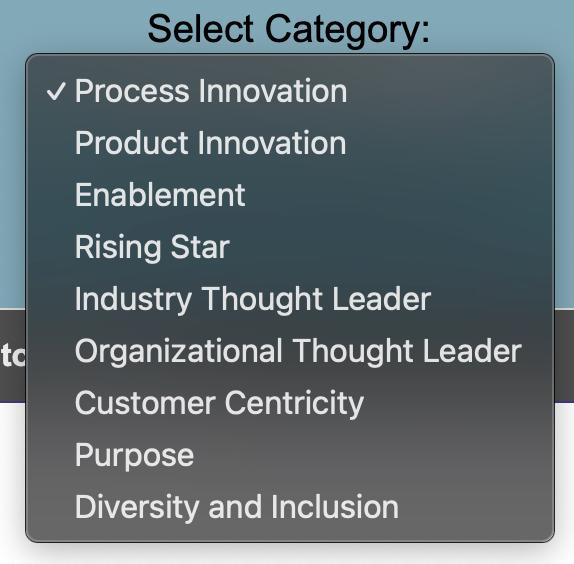
\includegraphics[width=0.5\textwidth]{img/categories.jpeg}
    \caption{Dropdown menu for selecting a category.}
    \label{fig:categories}
\end{figure}

\begin{figure}[H]
    \centering
    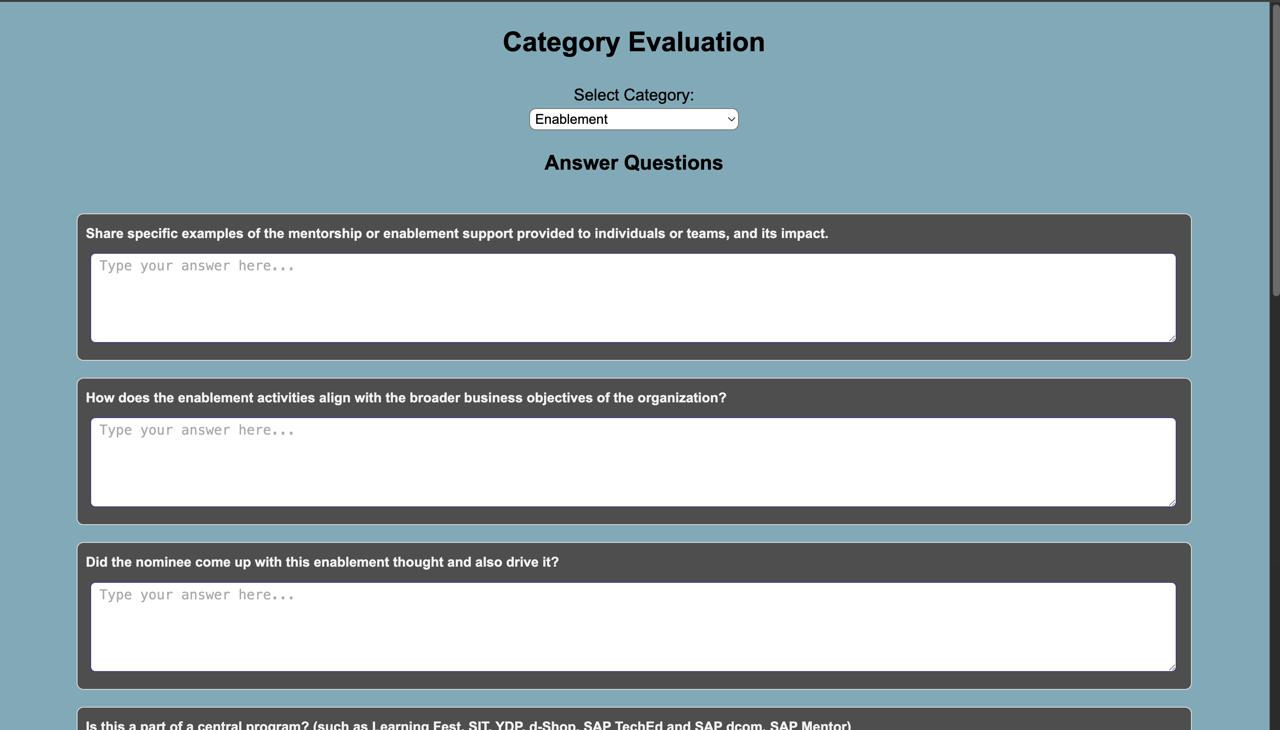
\includegraphics[width=0.9\textwidth]{img/empty.jpeg}
    \caption{Initial view of the page with the "Enablement" category selected.}
    \label{fig:empty}
\end{figure}

\subsection{Questionnaire Completion and Submission}
Once the user has answered all questions, they can submit their responses for evaluation. 
Figure~\ref{fig:submit} shows the bottom of the page, where the last few questions are answered and the "Submit" button is displayed.

\begin{figure}[H]
    \centering
    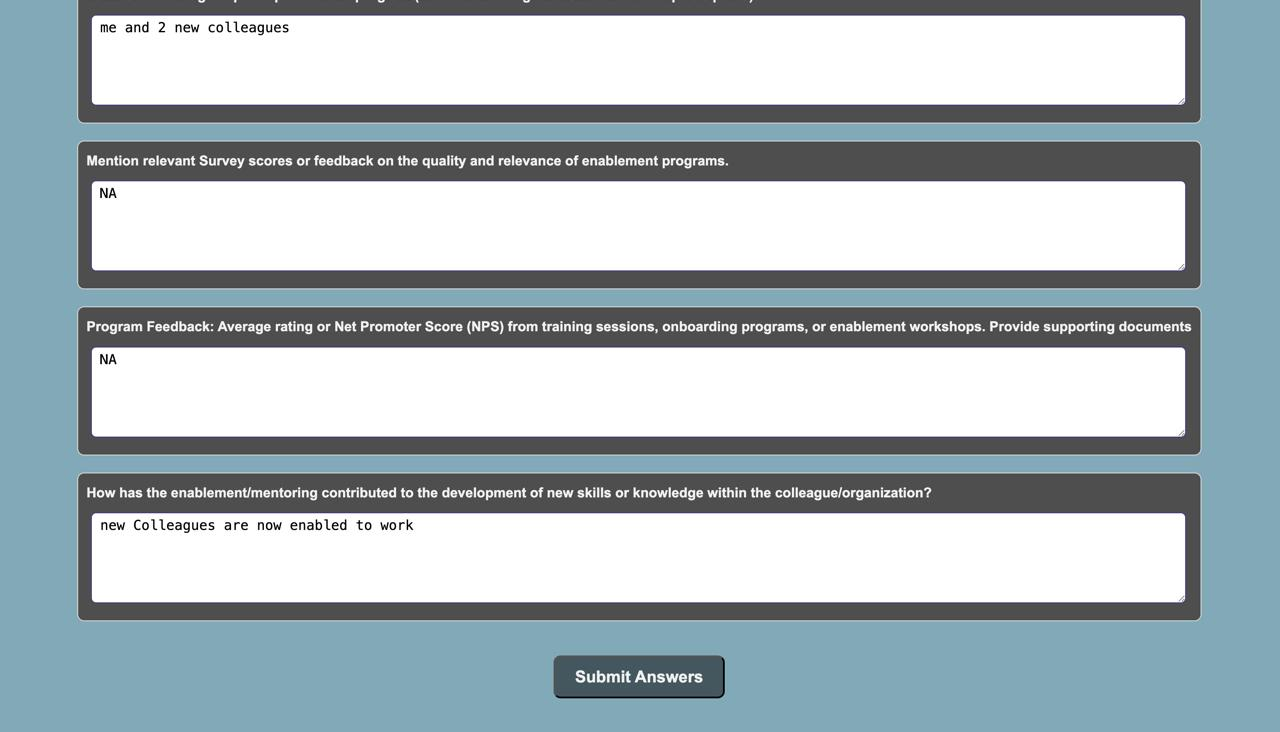
\includegraphics[width=0.9\textwidth]{img/submit.jpeg}
    \caption{Final view of the questionnaire before submission.}
    \label{fig:submit}
\end{figure}

\subsection{Evaluation Outcomes}
After submission, the \ac{LLM} evaluates the achievement based on the criteria defined for the selected category. 
Two examples are provided below, demonstrating both a failed and a successful submission for the "Enablement" category.

\subsubsection{Failed Submission}
Figure~\ref{fig:fail} shows the evaluation result for a failed submission. The achievement failed with a score of 3 due to not meeting the inclusion criteria and falling under the exclusion criteria. 
As specified in Listing~\ref{lst:enablement_criteria}, intra-team training and coaching a new joinee are excluded from consideration for this category.

\begin{figure}[H]
    \centering
    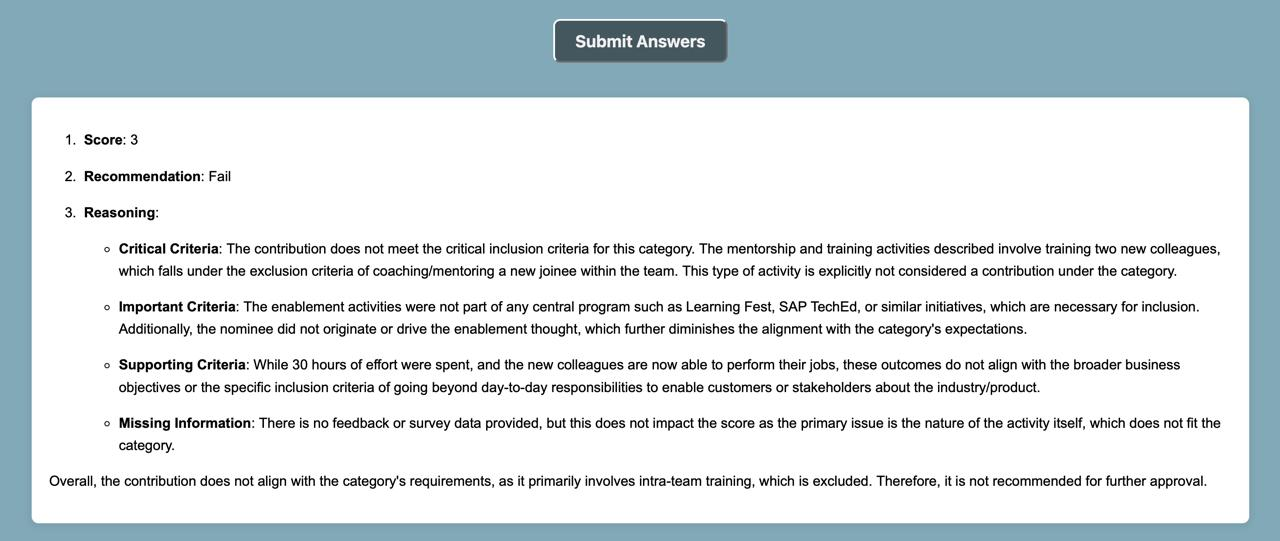
\includegraphics[width=0.9\textwidth]{img/fail.jpeg}
    \caption{Evaluation result for a failed submission under the "Enablement" category.}
    \label{fig:fail}
\end{figure}

\subsubsection{Successful Submission}
In contrast, Figure~\ref{fig:pass} shows a successful submission for the "Enablement" category. The achievement scored 7 and received a "Pass" recommendation. 
This submission involved creating worksheets and assisting with a Young Developers Program (YDP) event, aligning with the inclusion criteria. 
Additional factors that contributed positively were the nominee's 15 hours of effort and positive feedback received.

\begin{figure}[H]
    \centering
    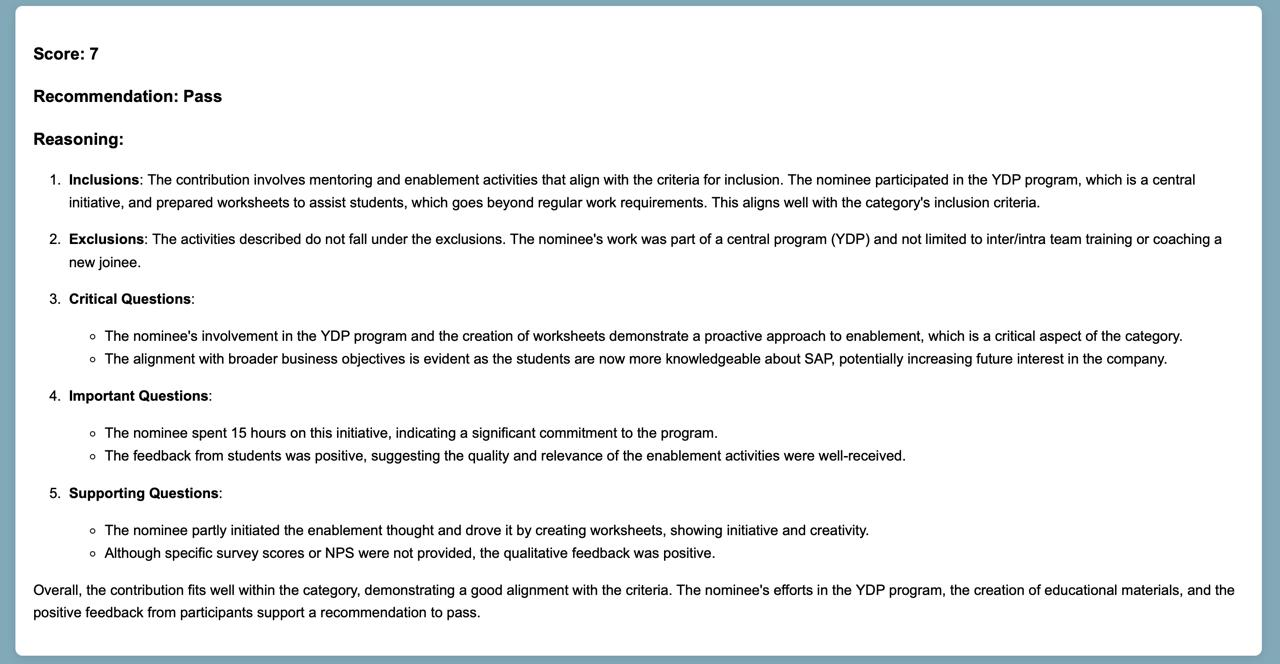
\includegraphics[width=0.9\textwidth]{img/pass.jpeg}
    \caption{Evaluation result for a successful submission under the "Enablement" category.}
    \label{fig:pass}
\end{figure}

\subsection{Prompt Debugging}
For transparency and debugging purposes, the application logs the user prompt sent to the \ac{LLM}. Figure~\ref{fig:prompt} displays the terminal output for the successful submission, 
showing the evaluation criteria, questions, and user responses. Note that the system prompt used during evaluation can be found in Listing~\ref{lst:evaluation_instructions}.

\begin{figure}[H]
    \centering
    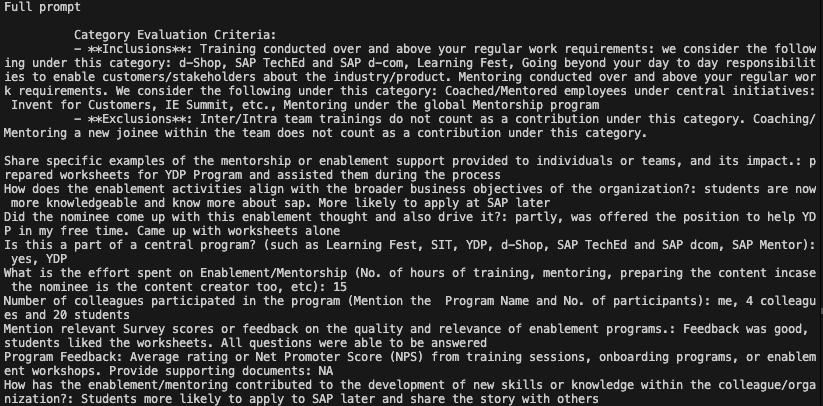
\includegraphics[width=0.9\textwidth]{img/prompt.jpeg}
    \caption{Terminal output showing the user prompt for a successful submission.}
    \label{fig:prompt}
\end{figure}